%% Intended to be included into a larger document
\chapter{Related Works}

%% Add more to introduce topics in this chapter?
\section{Defining Gamification}
Although gamification is a popular word nowadays, there are quite a few definitions came from different fields. Marketing industry defines gamification as integrating game dynamics into your site, service, community, content or campaign in order to drive participation. Wikipedia defines gamification as the use of game play thinking and mechanics to solve problems and engage audiences. They all seems evolve gamification with the goal of engagement. Some others considers any game related application is gamification, including serious game, playful interaction and game-based technologies.

Researcher Sebastian Deterding [ref] proposes an academic definition: Gamification is the use of game design elements in non-game contexts. It consists of 4 components:

\textbf{1. Game}: It is different than playful interaction, playful design. 

\textbf{2. Element}: It is not the complete game such as a serious game.

\textbf{3. Non-game Context}: Similar to serious game, it uses game for other purposed than game's normal expected use for entertainment.

\textbf{4. Design}: It is not game-based technologies or practices of wider game ecology.

Figure 2.1 illustrates the distinction with serious games and playful interaction.

\begin{figure}[htbp]
	\centering
		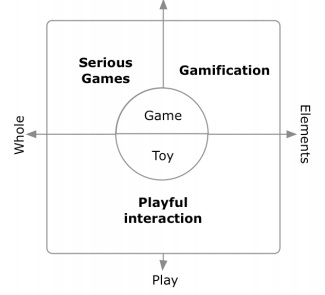
\includegraphics[scale=0.55]{defining_gamification.jpg}
		\caption{Defining Gamification}
		\label{fig:define_gamification}
\end{figure}

\section{Gamification Examples}
There are many examples of application that effectively employs game design elements. We will only briefly discuss a few here for the purpose of better understanding the gamification concept and how it is utilized across a wide range of everyday life.

\subsection{FourSquare : Check-in to Unlock}
FourSquare is a location-based game-like service  where players check-in to locations for virtual points and rewards. It is probably the most recognized forerunner of applying game mechanics to location-based networking application and made badges rewarding a common practice in most of catch-up gamified applications. Foursqure proved that simple game mechanics can affect behavior that can engage 10 million customers and being a successful business model.  By employing gamification elements such as points, badges, levels and leaderboards, it engages users to revisit a location such as restaurant or pub and become a loyal customer and finally the "major" of the place.  Some virtual rewards such as the "mayors" of Starbucks or certain badges could be converted into real products, e.g. a free coffee.
\begin{figure}[htbp]
	\centering
		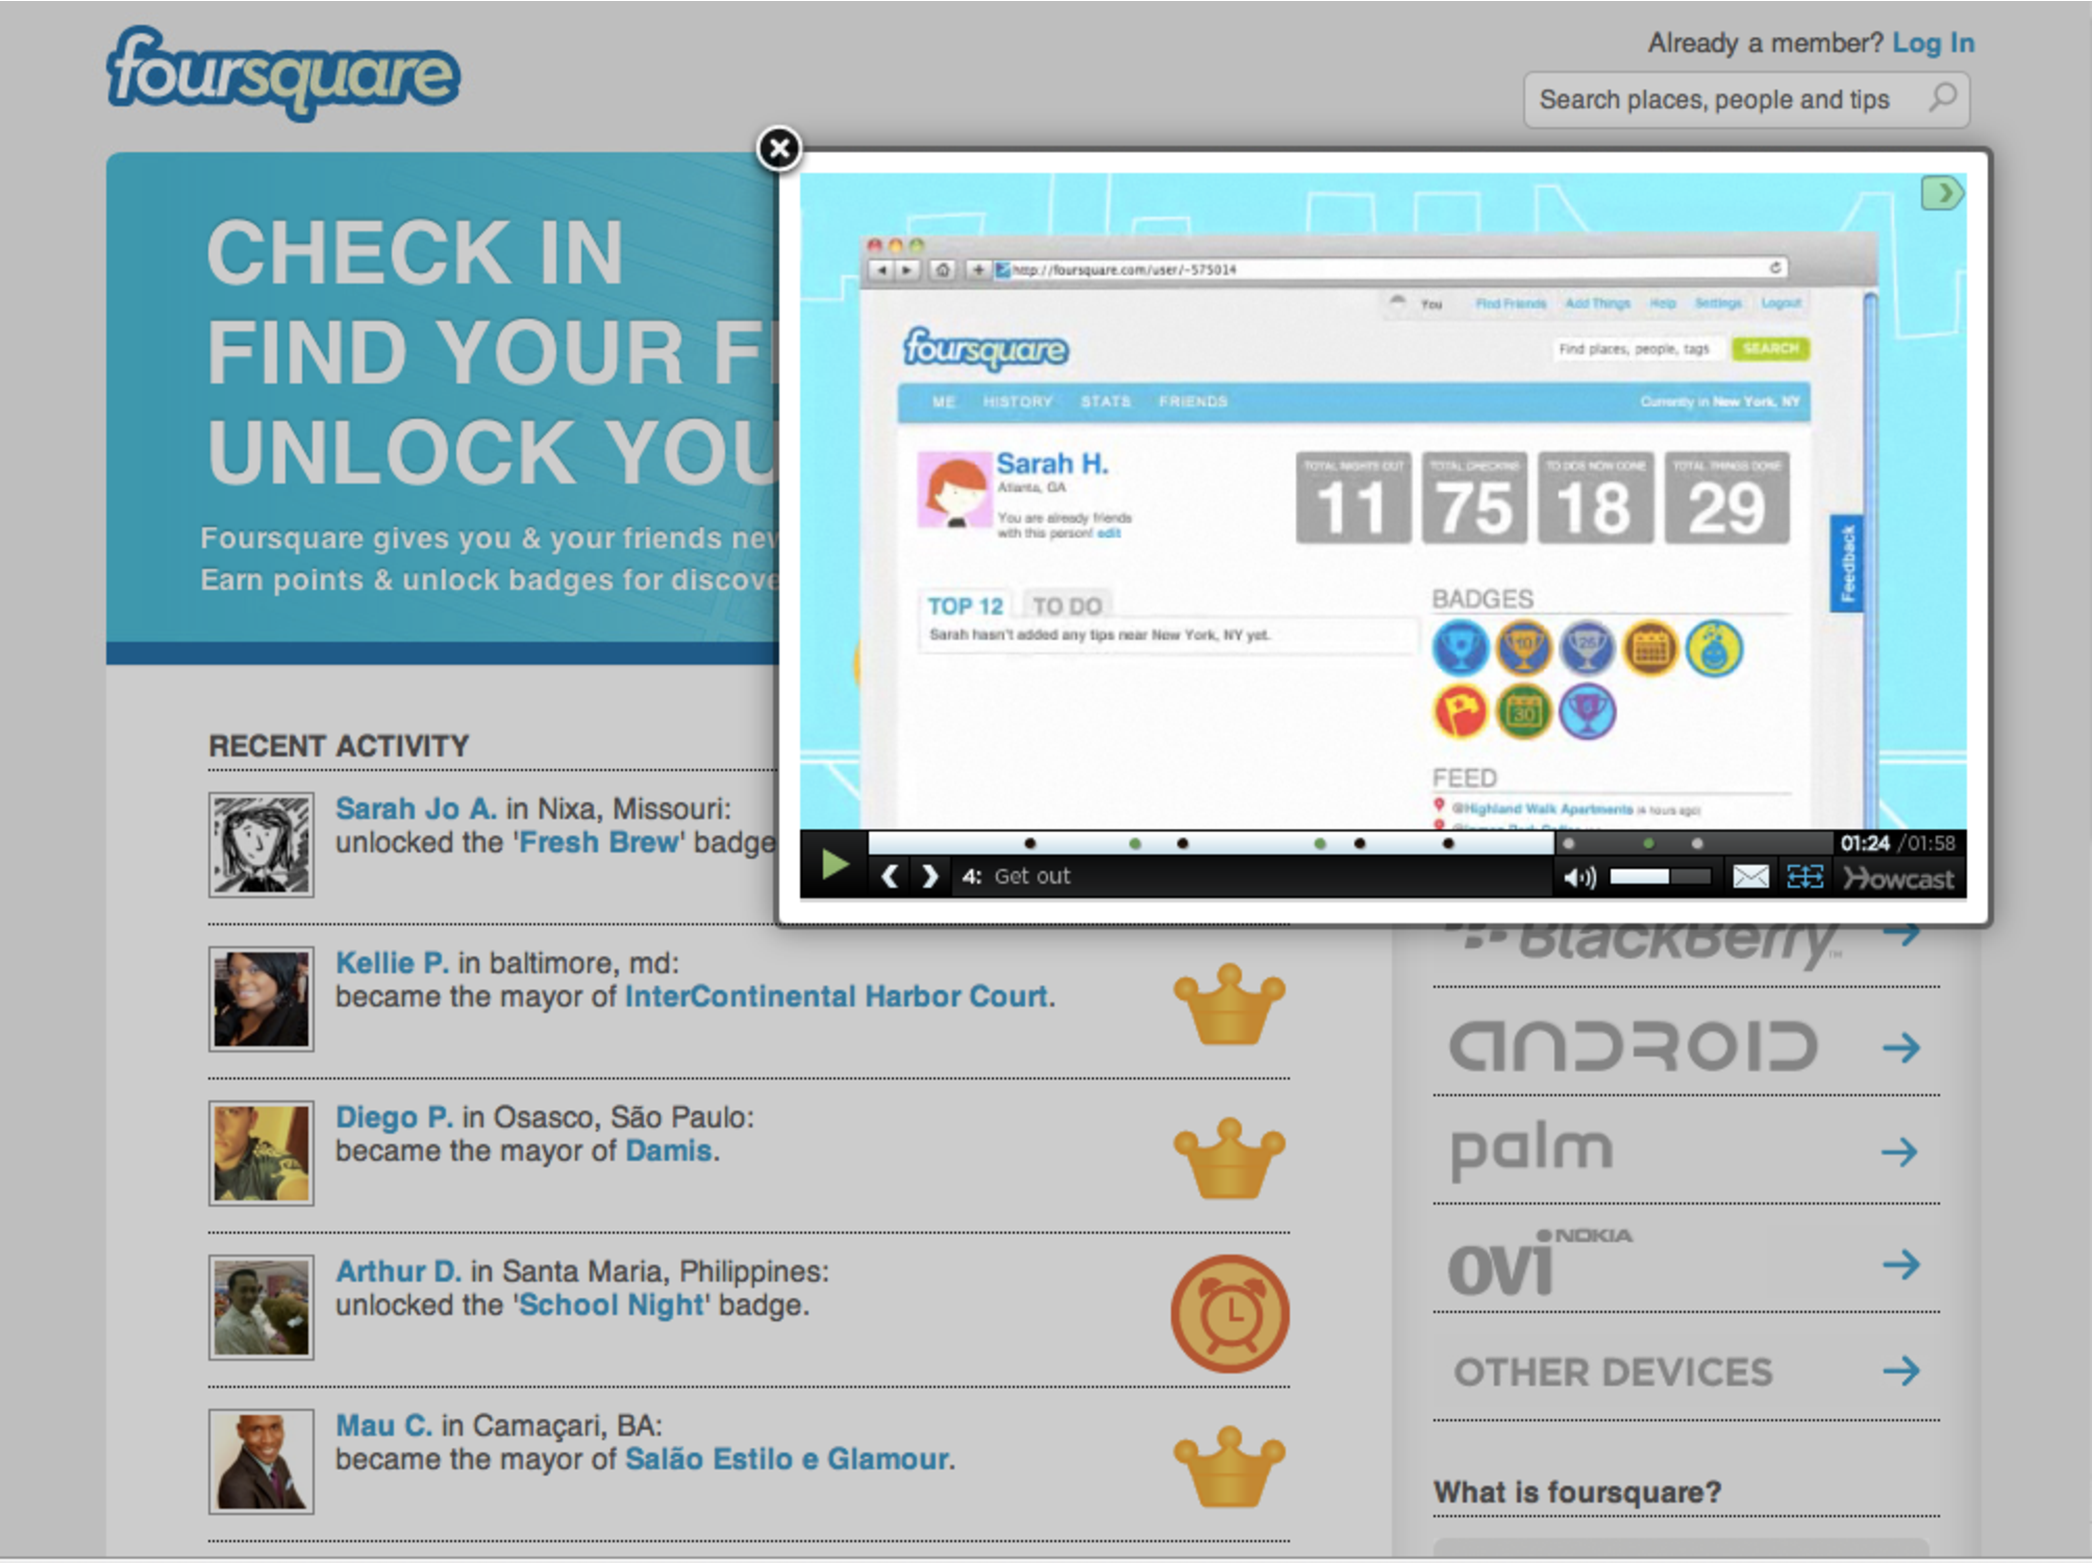
\includegraphics[scale=0.4]{foursquare.pdf}
		\caption{Foursquare makes modern badges popular}
		\label{fig:foursquare}
\end{figure}

\subsection{Nike+: Making Fitness Fun}
Nike+ is a social running game-like service that employs game mechanics to encourage runners - both casual and hardcore - to compete and improve their fitness, with the goal to solve the main problem of fitness program: motivation. Nike+ makes it easy for runners to upload their run data to the website and start challenging themselves and their friends, they can also get supports from their friends. 

\begin{figure}[htbp]
	\centering
		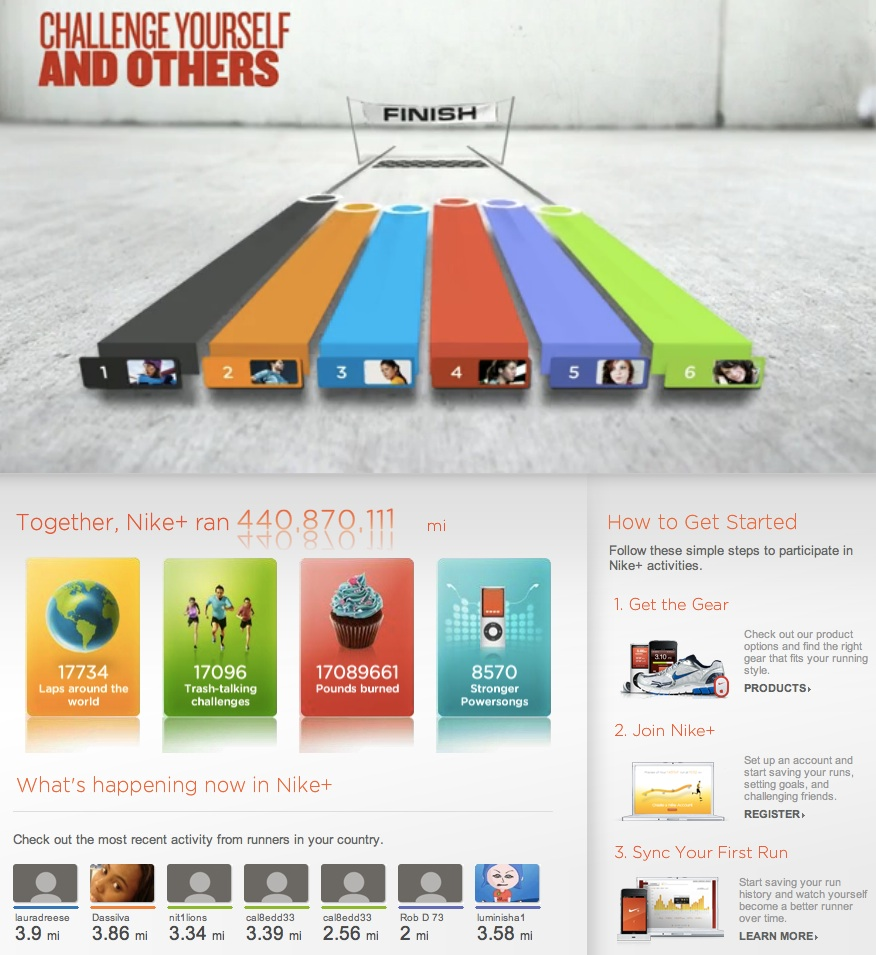
\includegraphics[scale=0.45]{nikeplus.jpg}
		\caption{Nike+ makes fitness run}
		\label{fig:nikeplus}
\end{figure}

\subsection{Microsoft RibbonHero - Making You Better Your Job} 
RibbonHero is a game that helps users discover new Microsoft Office features in a fun and motivating way. The goal is to have users build familiarity and expose them to the Office UI, so that they understand what kind of features are available, which according to the belief that Office "has a lot of powerful features that users might not know but can be really useful". The game gave users a chance to game experience with software outside of typically dry IT training videos. 

\begin{figure}[htbp]
	\centering
		\subfigure[Quest to earn points]{\label{fig:Ribbon1}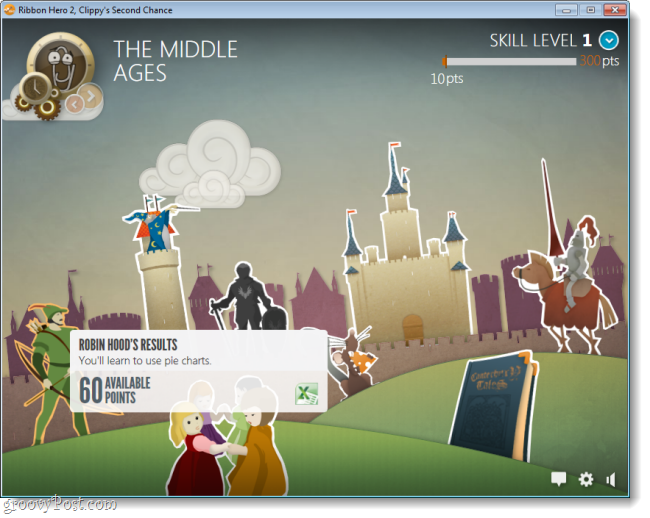
\includegraphics[height=2.5in]{ribbon1.png}}
		\subfigure[Competing a task]{\label{fig:Ribbon2}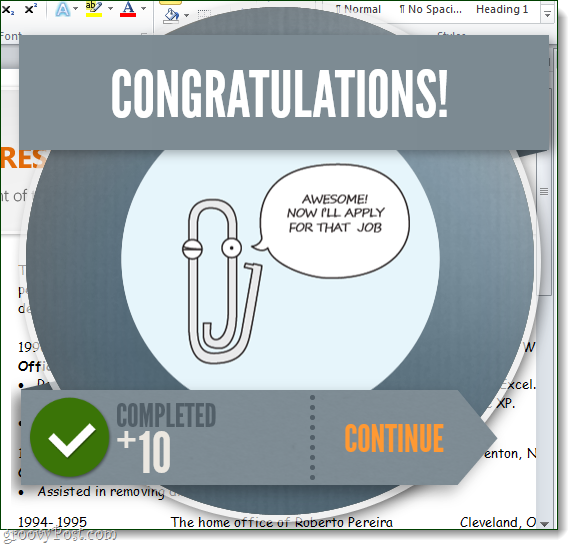
\includegraphics[height=2.5in]{ribbon2.png}}
		\caption{RibbonHero Helps to Learn Office}
		\label{fig:ribbon}
\end{figure}

\subsection{Mozilla - Open Badges}

\subsection{RecycleBank - Making the World Sustainable}
RecycleBank introduces a series of "Green Challenges" that used gaming techniques to motivate participants to learn about green living and to take small green actions to live more sustainable lives.  49,000 individuals participated in the "Green Your Home Challenges". Partnered with Google Analytics and ROI research, they found that:
\begin{itemize}
	\item Gamification can increase awareness of positive environmental actions. 97\% of participants surveyed said the game increase their knowledge of environment.
	\item Games can drive individuals to take positive social and environmental actions. Most participants surveyed indicated they are very or extremely likely to take green actions as a result of participating in the challenge. 
	\item Games are an effective and appealing educational tool. 86\% participants agreed online games and contest can be a good way to inform and educate them personally. 
\end{itemize}

\begin{figure}[htbp]
	\centering
		\subfigure[Green Your Home Challenge]{\label{fig:RecycleBank1}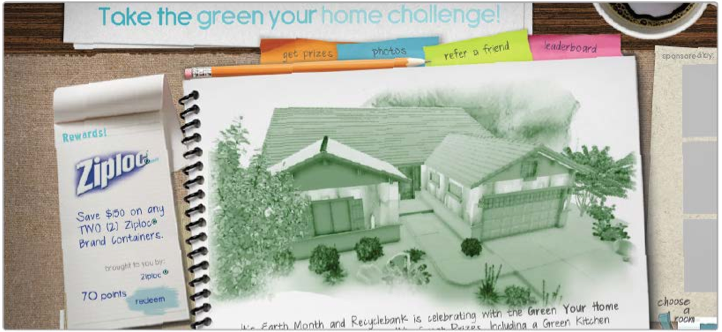
\includegraphics[scale=0.3]{recyclebank1.png}}
		\subfigure[Game Change Behavior]{\label{fig:RecylceBank2}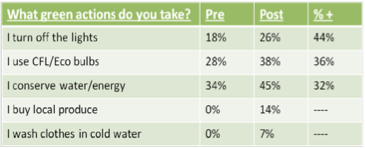
\includegraphics[scale=0.65]{recyclebank2.png}}
		\caption{RecycleBank - Gaming for Good}
		\label{fig:ribbon}
\end{figure}	
	
\section{Why Games}
\label{sec:why-games}

Gamification is not about games, in fact as a subject gamification is deals with everything else but games. But the research in gamification have to largely base on the studies of games. The games already prove to be an effective engaging media and ubiquitous as every day life. In fact, "video game is everywhere" is the critical thesis of many gamification advocates. 

[need more data on game market, player demography]

The following sections will examine a few most popular games and genre to understand what game mechanics give games such power nowaday.

\subsection{Ancient Game}

\subsection{Modern Game}

\subsection{Casual Game: Angry Birds}
In today's tech world, no gaming platform is completed without the new star game Angry Birds. There  are over 50 million individuals have downloaded this simple game. The total number of hours consumed by world-wide players is roughly 200 million minutes a day, that is 1.2 billion hours a year.  According to Neiman Journalism Lab[ref], all person-hours spent creating and updating the entire wikipedia totals about 100 million hours.  That is half day of the Angry Birds play time. Why is this seemly simple game so massively compelling? Charles Mauro [ref] discussed the cognitive teardown of Angry Birds in Human factor engineering (aka usability engineering) for the sake of answering the more "important" real world question, "why users don't find their company's software or product engaging?":

    * Simple Engaging Interaction Concept:
    Angry Birds' simple interaction model is easy to learn and incremental increase of complexity.

    * Cleverly managed response time: 
    In Angry Birds design, it is not "faster is better", instead, different birds have different trajectory time and the flight path of the bird is intentionally illustrated. It solved one huge problem for user interfaces - error correction.It also take a seemly long time for the pigs to expire once their hours are collapsed, this non-functional time delay increases the playfulness of the game and bring users entertainment.

\subsection{Social Game: Zynga-Ville}
With the motto  "Connecting the world through games", Zynga who found in 2007 quickly become the top game company catching up to the more traditional establishment such as EA and Activision Blizzard. With the help of socal network platform Facebook, the FarmVille and CityVille quickly become the most popular games within Facebook. Zynga later expanded the games into other platform such as mobile and  new google+ social network. 

[more research on Zynga's game number, total time played, total player, compared to Angry Birds]

http://www.philmichaelson.com/user-generated-content/8-design-tactics-farmville/

FarmVille has 71 million active users while Twitter has around 22 million active users (Twitter has 110 million registered users, of which an estimated 20\% are likely active).  Perhaps more impressively, Zynga is estimated to generate \$50 million in revenue from the most engaged members who buy virtual goods and keep up a toolbar.

8 Ways FarmVille Designs for Engagement

1. Reward users for returning in a short time period. 

2. Reward users for helping friends every day.

3. Allow users to create without typing. 

4. Show progress�everywhere�on everything.

5. Make users feel lonely without friends�because if they get friends on, they�ll stay longer.

6. Enable self expression. 

7. Offer increasing levels of complexity for mastery. 

8. Have surprises and limited time events.

Questions: Will they still have more active users than Twitter in 2 years?

One distinct characteristic of Zynga games is that they are social and they are all interconnect through an exchangable virtual currency "Zynga Points". 

[more on virtual currency's social effect]

\subsection{MMORPG: World of Warcraft}

\section{Game Motivation}
Researchers from Physcology, game industries and acamedic, have studied the psychology of motivation that makes online games so engaging. Online games are voluntary experiences that become so addictive that "people [who play them] won't even go to the bathroom [in the middle of a game]," Rigby pointed out. 

\subsection{Flow}
Psychology professor Mihaly Czikszentmihalyi introduced a specific kind of happiness that he named "flow", which is widely accepted to be one of the fundamental reasons that people play games. Flow, a state of absorption in one's work, is characterized by intense concentration, loss of self-awareness, a feeling of being perfrectly challenged (neither bored nor overwhelmed) and a sense that time if flying. 

As Csikszentmihalyi describes (Csikszentmihalyi 1990), there are seven core components of flow that are summarized in Table 2.1. These components can be broken into two categories: conditions and characteristics. Conditions must be achieved before flow can be reached. Characteristics occur while a person is in flow, even though they may be unaware of it.

\begin{table}[htbp]
  \centering
    \caption{Flow Condition and Characteristics}
    \begin{tabular}{ | l | p {10cm} |}
    \hline
    Conditions of Flow & Explanation \\ \hline
    Clear tasks & Person understands what they must complete  \\ \hline
    Feedback & Person receives clear and immediate feedback showing what succeeds and what fails \\ \hline
    Concentration/focus & Person is not distracted and can fully attend to the task \\ \hline
    An attainable, balanced goal & Goal is challenging and within their abilities to complete \\ \hline
    Characteristics of Flow & Explanation \\ \hline
    Control & Person believes their actions have direct impact on tasks and that they can control the outcome \\   \hline
    Diminished awareness of self & Complete focus on the task leaves little room for feeling self-conscious or doubt. Often described as becoming a part of the activity. \\ \hline
    Altered sense of time & Perception of time is distorted. Seconds can feel like minutes, minutes like hours. Yet, time also passes by quickly, unnoticed. \\ \hline
    \end{tabular}
\end{table}

In order to achieve the flow, the right conditions above must exist. The last and the most important condition is a balanced goal that is challenging yet achievable within the individaul's ability. A task that is not challenging or  requires excessive time to complete becomes boring and players lose interest; A task that is too hard causes frustration and anxiety and again players lose interest. With a person’s skills improve over time, the challenge needs to increase along with the improving skills. This balance is referred to as the flow channel as shown in figure 2.1 (based on a diagram from Csikszentmihalyi, 1990, p 74).

\begin{figure}[htbp]
	\centering
		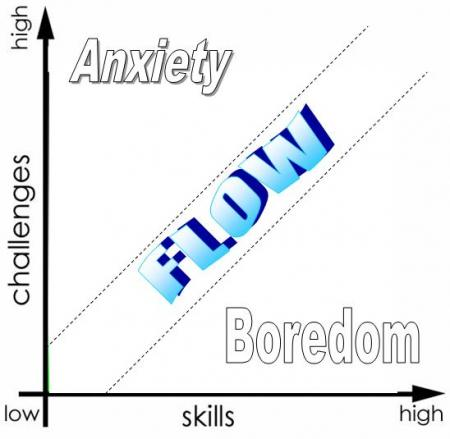
\includegraphics[scale=0.59]{czikszentmihalyi.jpg}
		\caption{The state of flow is achieved between anxiety and boredom}
		\label{fig:state_of_flow}
\end{figure}

\subsection{Player Type}
In order to understand why people play games, Ricahrd Bartle identified four player personality types by studying players of MMOGs (massively multiplayer online games), as shown in Figure 2.2

\begin{figure}[htbp]
	\centering
		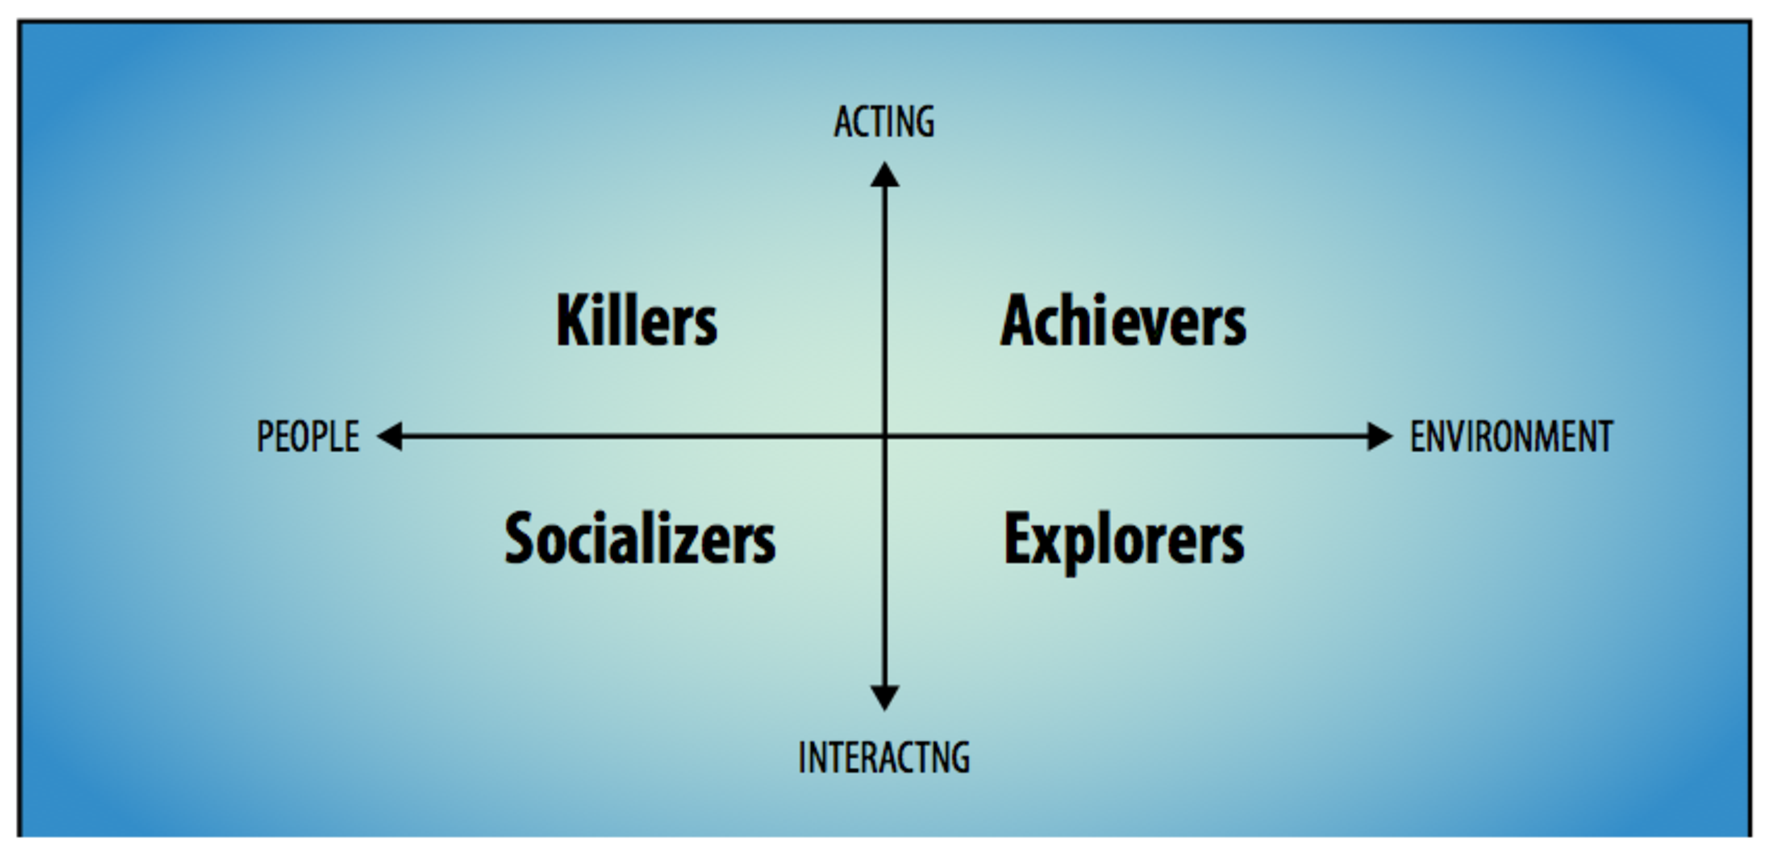
\includegraphics[scale=0.59]{bartle_player_type.pdf}
		\caption{Bartle's Player Types}
		\label{fig:player_types}
\end{figure}

1. Explorers have a clear inclination towards discovery

2. Achievers are definitely motivated by the accumulation of experience points, status and ranks associated with their proficient use of the software

3. Killers are motivated by challenge, competition, and the rapid pace of usage as in a first-person shooter game.

4. Socializers like to socialize in a collaborative non-confrontational environment.
 
One study [ref?] found that approximately 80\% of the populations are Socializers. Explorers, achievers and killers make up only about 20\% of the population.

\subsection{Fogg Behavior Model}
Stanford University's researcher BJ Fogg [ref] introduces the Fogg Behavior Model (FBM) to explain what causes behavior change. The model shows that three elements, Motivation, Ability, and Trigger must converge at the same moment for a behavior to occur. 

\begin{figure}[htbp]
	\centering
		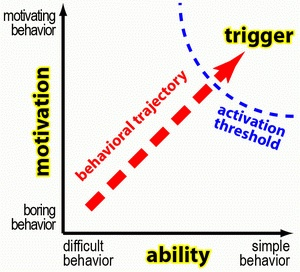
\includegraphics[scale=0.59]{fogg_behavior_model.jpg}
		\caption{Fogg Behavior Model}
		\label{fig:behavior_model}
\end{figure}

1. Motivation: the person wants desperately to perform the behavior (i.e. he is highly motivated)

2.Ability: the person can easily carry out the behavior (i.e. he considers the behavior very simple)

3. Trigger: the person is triggered to do the behavior (i.e. he is cued, reminded, asked, called to action, etc.)
 
Michael Wu [ref] uses FBM to analyze why and how gamification are able to drive actions. 
"Game mechanics and game dynamics are able to positively influence human behavior because they are designed to drive the players above the activation threshold (i.e. the upper right of the ability-motivation axis), and then trigger them into specific actions. In other words, successful gamification is all about making these three factors occur at the same time."

\section{Game Design Framework}
\subsection{Mechanics/Dynamics/Aesthetics(MDA)}
A framework introduced by game designer Marc LeBlanc describes three pillars of a good game:

Mechanics: The rules and concepts that formally specify the game-as-system. They make up the functioning components of the game.

Dynamics: The run-time behavior of the game-as-system, They are the player's interactions with mechanics.

Aesthetics: The desirable emotional responses evoked by the game dynamics. They are how the game makes the player feel.

\section{Game Mechanics}
There are many game mechanics and dynamics make game a game. 

\begin{table}[htbp]
  \centering
    \caption{Mega List of Game Mechanics and Benefits}
    \begin{tabular}{ | l | p {8cm} | p {4cm} | p {2cm} |}
    \hline
    Types & Mechanics / Examples & Benefits & Personality Types \\ \hline
	Progression & Achievements: normally represents as badge, completed something & Engagement, Loyalty, Time Spent, Influence, Fun, SEO, UGC & Achievers, Explorers, Killers \\ \hline
	Progression & Levels: a system of reward for a cumulation of points, Often are unlocked as players progress to higher levels. & 	Engagement, Loyalty, Influence, Time Spent, Virality, Fun & Achievers, Explorers, Killers \\ \hline
	Progression & Points: a running numerical value given for any single action or combination of actions. & Engagement, Loyalty, Influence, Time Spent, Virality, Fun, UGC & Achievers, Explorers, Killers \\ \hline
	Progression & Progression: success is granularly displayed and measured through the process of completing itemized tasks, such as a progress bar. & Engagement, Loyalty, Influence, Time Spent, Fun, UGC & Achievers, Killers \\ \hline
	Feedback & Appointment Dynamics: at a predetermined times/places a user must return for a positive effect & Engagement, Influence, Time Spent & Archivers, Explorers, Socializers \\ \hline
	Feedback & Bonuse: a reward after having completed a series of challenges or a specific task & Engagement, Influence, Time Spent, Virality, Fun, UGC & Archivers, Explorers, Socializers, Killers \\ \hline
	Feedback & Cascading Information Theory: information should be released in the minimum possible snippets to gain the appropriate level of understanding & Engagement, Loyalty, Influence, Time Spent & Archivers, Explorers, Socializers, Killers \\ \hline
	Feedback & Combos: reward skill through doing a combination of things, usally comes with the reward of a bonus & Engagement, Influence, Time Spent, Virality & Archivers, Explorers, Socializers, Killers \\ \hline
	Feedback & Countdown: players are only given a certain amount of time to do something. This will create an activity graph that causes increased initial activity increasing frenetically until time runs out, which is a forced extinction. & Engagement, Fun, Influence & Achievers, Explorers, Killers \\ \hline	
	Feedback & Quests/Challenges: Challenges usually implies a time limit or competition whereas Quests are meant to be a journey of obstacles a player must overcome. a way to organize player effort. & Engagement, Loyalty, Revenue, Influence, Time Spent, Virality, SEO, Fun, UGC & Achievers, Explorers, Killers \\ \hline
	Feedback & Reward Schedules: The fixed or variable timeframe and delivery of the rewards, contingency, response, reinforcer. & Engagement, Loyalty, Revenue, Influence, Time Spent, Virality, SEO, Fun, UGC & Achievers, Explorers, Killers \\ \hline
	Behavioral & Discovery/Exploration: players love to discover and to be surprised. & Engagement, Loyalty, Influence, Time Spent, Fun & Explorers, Achievers \\ \hline
    \end{tabular}
\end{table}

\begin{table}[htbp]
  \centering
    \caption{Mega List of Game Mechanics and Benefits, Continue}
    \begin{tabular}{ | l | p {8cm} | p {4cm} | p {2cm} |}
    \hline
    Types & Mechanics / Examples & Benefits & Personality Types \\ \hline	
	Behavioral & Epic Meaning: Players will be highly motivated if they believe they are working to achieve something great, something awe-inspiring, something bigger than themselves. & 	Engagement, Loyalty, Influence, Time Spent, Fun & Achievers, Explorers, Socializers, Killers \\ \hline
	Behavioral & Free Lunch: getting something for free due to someone else having done work. Groupon & Engagement, Loyalty, Revenue, Influence, Virality, Fun & Achievers, Explorers,  Socializers, Killers \\ \hline
	Behavioral & Infinite Gameplay: do not have an explicit end, static state is its own victory. & 	Engagement, Loyalty, Revenue, Influence, Time Spent, Fun & Achievers, Killers \\ \hline
	Behavioral & Loss Aversion: influences user behavior not by reward, but by not instituting punishment. the player having to perform an action to avoid losing something they currently have. & Engagement, Loyalty, Influence, Time Spent, Virality, Fun & Achievers, Explorers \\ \hline
	Behavioral & Lottery:  the winner is determined solely by chance. winners will generally continue to play indefinitely while losers will quickly abandon & Engagement, Loyalty, Revenue, Influence, Time Spent, Virality, Fun & Achievers, Explorers, Socializers, Killers \\ \hline
	Behavioral & Ownership: creates Loyalty by owning things. & Engagement, Loyalty, Revenue, Influence, Time Spent, Virality, SEO, Fun, UGC & Achievers, Explorers, Socializers, Killers \\ \hline
	Behavioral & Community Collaboration: an entire community is rallied to work together to solve a riddle, a problem or a challenge. Immensely viral and very fun. & 	Engagement, Influence, Time Spent, Virality & Archivers, Explorers, Socializers \\ \hline
	Behavioral & Behavioral Momentum: a tendency of players to keep doing what they have been doing & Engagement,  Loyalty, Revenue, Influence, Time Spent & Archivers, Explorers, Socializers, Killers \\ \hline
	Behavioral & Blissful Productivity: playing hard rather than relaxing makes you happier  & Engagement & Archivers, Explorers, Socializers, Killers \\ \hline
	Behavioral & Status: The rank or level of a player. Players are often motivated by trying to reach a higher level or status. Also relates to envy. & Engagement, Loyalty, Revenue, Influence, Time Spent, Virality, SEO, Fun, UGC & Achievers, Socializers,Killers \\ \hline
	Behavioral & Urgent Optimism: The desire to act immediately to tackle an obstacle combined with the belief that we have a reasonable hope of success. & Engagement, Fun & Explorers, Killers \\ \hline
	Behavioral & Virality: more successful in the game if you invite your friends, the social check-in. & Engagement, Loyalty, Revenue, Virality, SEO, UGC & Socializers, Achievers,Killers \\ \hline
    \end{tabular}
\end{table}

\section{Game Elements}

\begin{table}[htbp]
  \centering
    \caption{List of Game Elements}
    \begin{tabular}{ | l | p {12cm} |}
    \hline
    Elements & Description and Examples \\ \hline
	Activity Feed & shows players what has been taking place in the system overall and motivate the player to obtain the same achievement as others. \\ \hline
	Avatars & unique representations for a player. shows a high emotional attachment between the player and the game. often customization and decoration are enhancement for higer engagement. \\ \hline
	Easter Eggs & an intentional hidden message, in-joke. \\ \hline
	Instances & are created for players to have a unique experience that is outside the normal experience. When a player creates a special unique page experience that allows to log into and view their unique content an instance has been created. \\ \hline
	Leaderboards & are a means by which users can track their performance, subjective to others. Leaderboards visually display where a user stands in regards to other users. Leaderboards can be broken down into several subcategories such as: Global, Friends, Relative, Isolated etc. \\ \hline
	The Notifier & is a direct way to give the user direct feedback about their progress, change of status in the gameplay experience etc. \\ \hline
	User Profile & displays a User's data about their activity on a website and can be used to tell the world and a community on the internet who they are. \\ \hline
    \end{tabular}
\end{table}

\section{Gamification Debates}

Debate continues over whether gamification itself is inherently good or bad. That is, is its use motivated by bad intentions to dupe people into doing things that aren't necessarily in their best interest? Or are some attempts at gamification merely poorly executed, so that its effects are superficial and fail to transform people's behavior in long-lasting, positive ways? "If gamification is fundamentally about tricking people to feel happier about situations that aren't going to be better [for them], then it's problematic on a lot of levels -- both ethically and in effectiveness in the long term," according to Kevin Werbach, a Wharton professor of legal studies and business ethics who organized the conference with Dan Hunter, a professor at New York Law School. "The question is: What are the aspects of [gamification] that are really about meaningfully improving people's experience?"

Gamification is naturally suspect if it is used by corporations, terrorist organizations or others with the intention of potentially causing harm -- whether to push the sales of useless products and services like subprime mortgages, or to lure recruits into suicide missions. Even if the goals of gamification are exemplary, however, does gamification merely gloss over real problems that require real answers? For example, does awarding participants points and using other incentives through the HopeLab program significantly impact the root causes of teen obesity in low-income neighborhoods, such as the lack of access to, and the high price of, fresh fruits and vegetables? By gamifying the problem, "you're spreading butter over toast so it tastes better, but it doesn't solve the problem," Georgia Tech's Bogost pointed out.

Current efforts at gamification come with other pros and cons, including the relative value of extrinsic motivators (such as points, badges and rewards) versus intrinsic motivators generated by an individual's internal will or desires. "In the long run, [extrinsic rewards] are not fun," said Nicole Lazzaro, Founder of XEODesign, which helps companies such as Sony, Sega and Leapfrog improve player experiences. "The use of extrinsic motivation will decrease motivation to use your products and services once you remove that reward.... You have to keep upping the dose to have the same motivation and change in behavior over time."

But Carnegie Mellon's Schell cautioned against writing off extrinsic rewards without a deeper understanding of the psychology behind motivation. "We don't fully grasp the complex relationship between intrinsic and extrinsic rewards," he noted. And extrinsic rewards can be a catalyst for intrinsic motivation, added Michael Wu, chief scientist of Lithium Technologies, a social networking research and consulting firm. "Using an extrinsic reward is a good way to get people to start doing something," he said. Although the outside incentive may be the initial reason that people adopted a particular activity, Wu suggested that they may ultimately develop internal motivators. Once teens start losing weight and looking better, spurred by the lure of HopeLab's Zamz currency, for example, they may embrace a healthier lifestyle because it makes them feel better about themselves.

In a field rife with anecdotes but little hard data, Wharton's Werbach and New York Law School's Hunter intend to develop in-depth case studies to examine the types of business problems organizations want gamification to solve, the techniques used and the results. According to Werbach, there currently are few bridges between game design as a craft and psychological research. "That's why research is valuable -- to get beyond whether gamification is good or bad, and does it work or not."
"

\subsection{Can you gamify a suicide hotline?}
Can you gamify everything? "No, you can not gamify game". According to Gabe Zichermann, the idea of baking game mechanics into everything you do is fun, but when asked how would you make a suicide hotline fun, he admitted that adding games to a suicide prevention seems distasteful at first, but he could add a game mechanics like a competitive environment in a call center setting.

\subsection{Gamification is bull*it}
At the Wharton conference, Georgia Institute of Technology professor and game designer Ian Bogost called gamification efforts "exploitation-ware" that is being "invented by consultants as a means to capture the wild, coveted beast that is video games and to domesticate it for use in the grey, hopeless wasteland of big business." Gamification, he argued, "gets games wrong, mistaking incidental properties like points and levels for primary features like interactions with behavioral complexity."

\subsection{Gamification vs Serious game}
Serious game are generally defined[ref], to include games that make use of computer technology and advanced video graphics and that are used for the purposes of learning and training.

\section{How to gamify}

\subsection{Gamification 1.0}

\subsection{Smart Gamification}
"Carnegie Mellon University professor and game designer Jesse Schell, who ignited much of the current interest in gamification with a keynote address at the 2010 Design Innovate Communicate Entertain (D.I.C.E.) Summit, said he was surprised people took interest in his presentation, since he had talked about the phenomenon for years with little response. "Something in the air crystallized at that time," he noted. "There is something that's happening in culture right now -- a shift just as sure as the Industrial Revolution was a shift. We're moving from a time when life was all about survival to a time when it was about efficiency into a new era where design is largely about what's pleasurable." According to Schell, gamification is a way to arrive at a "fundamental understanding of what it is that's pleasurable to people." What's more, online games have entered the mainstream, helped by platforms such as smartphones, tablets and Facebook."

\section{Gamification Service or Platform}
This section outlines the current industry players that provides gamifcation service via platforms or consultation service. [see figure 2.1]

\begin{figure}[htbp]
	\centering
		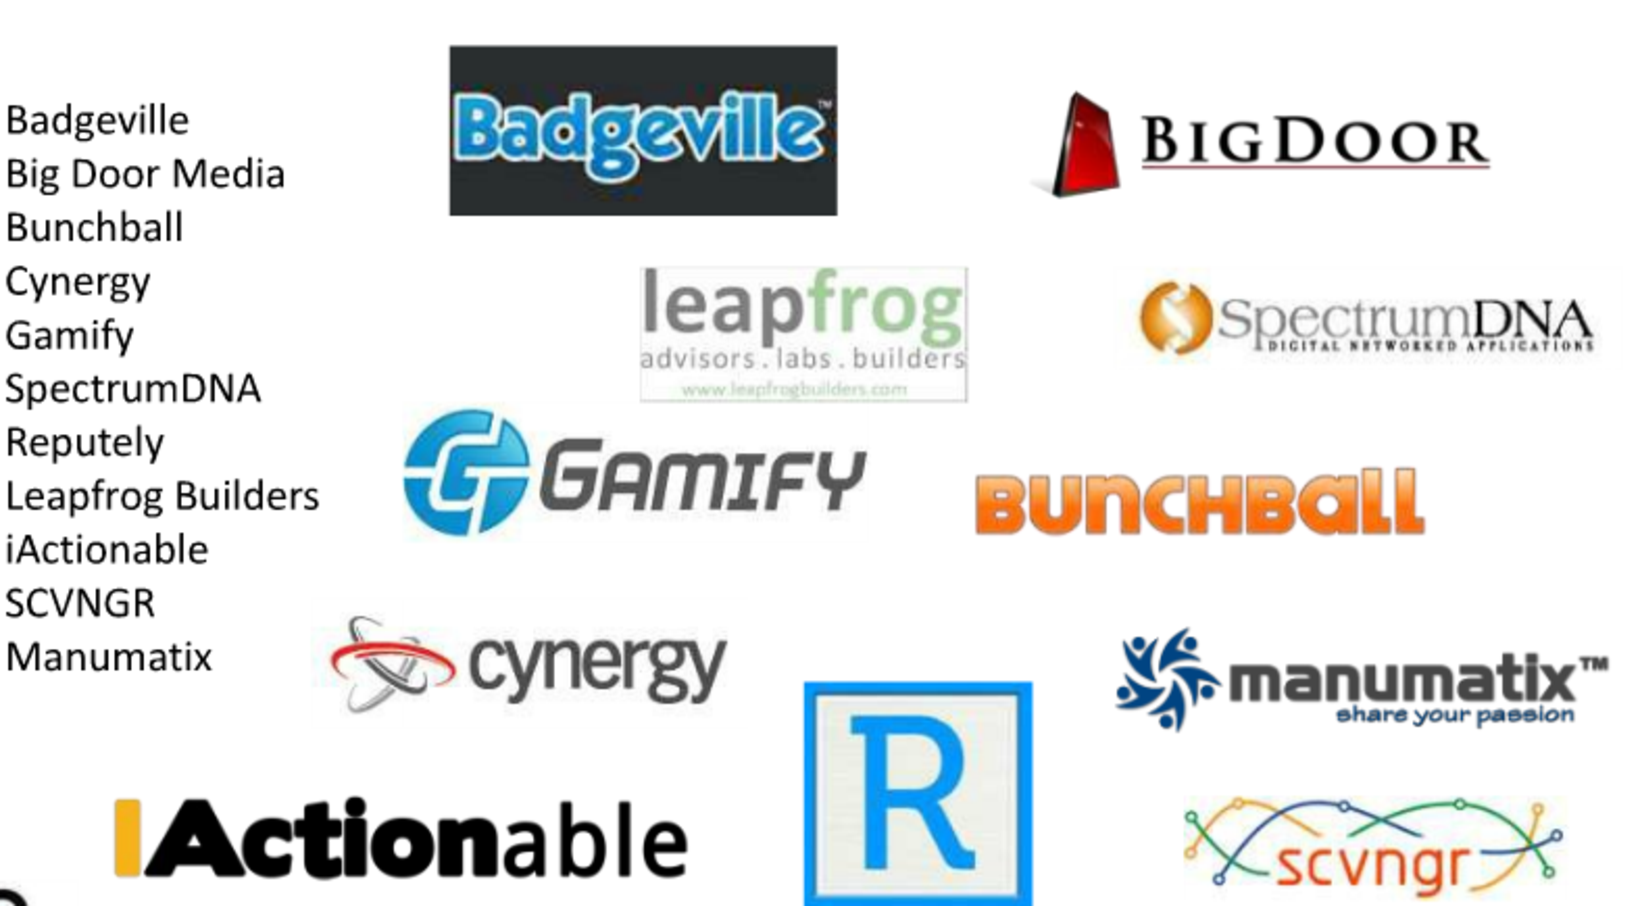
\includegraphics[scale=0.59]{gamification-service.pdf}
		\caption{Gamification Service Industry}
		\label{fig:gamification-service}
\end{figure}

\section{Gamification Analytics}
The objective evaluation of Player Experience (PX)[ref] in games is the goal of game metrics and analytics research. With the technology advancement, it is possible to automatically log numerical informations on in-game player behaviour and analyze them in different context. This methodology provides a qualitative and quantitative result of the player experience in games, which in turn affect the result of gamification.

source: top 10 social game metrics

1. Entry Event Distribution

2. Exit Event Distribution

3. Message/Post/Comments distribution

4. Message Click Through Rate

5. Engagement time

6. Revisit Rate

7. Virality (K-factor)  

8. Lifetime Network Value

9. Conversion to paying users

10. Average Revenue Per Paying User

from gamification.org/wiki Standard Engagement Metrics are:

Unique visitors

Page views per visitor

Time spent on site

Total time spent per user

Frequency of visits

Depth of visit

Participation

Conversions